\documentclass[11pt,letterpaper]{book}
%-----------------------PAQUTES---------------------------%
\usepackage{graphicx}
\usepackage[spanish]{babel}
%\usepackage{listings}
%\usepackage{color}
%------------------------MACROS---------------------------%
%\definecolor{mygreen}{rgb}{0,0.6,0}
\definecolor{mygray}{rgb}{0.5,0.5,0.5}
\definecolor{mymauve}{rgb}{0.58,0,0.82}

\lstset{ 
  backgroundcolor=\color{white},   % choose the background color; you must add \usepackage{color} or \usepackage{xcolor}; should come as last argument
  basicstyle=\footnotesize,        % the size of the fonts that are used for the code
  breakatwhitespace=false,         % sets if automatic breaks should only happen at whitespace
  breaklines=true,                 % sets automatic line breaking
  captionpos=b,                    % sets the caption-position to bottom
  commentstyle=\color{mygreen},    % comment style
  deletekeywords={...},            % if you want to delete keywords from the given language
  escapeinside={\%*}{*)},          % if you want to add LaTeX within your code
  extendedchars=true,              % lets you use non-ASCII characters; for 8-bits encodings only, does not work with UTF-8
  firstnumber=1000,                % start line enumeration with line 1000
  frame=single,	                   % adds a frame around the code
  keepspaces=true,                 % keeps spaces in text, useful for keeping indentation of code (possibly needs columns=flexible)
  keywordstyle=\color{blue},       % keyword style
  language=Octave,                 % the language of the code
  morekeywords={*,...},            % if you want to add more keywords to the set
  numbers=left,                    % where to put the line-numbers; possible values are (none, left, right)
  numbersep=5pt,                   % how far the line-numbers are from the code
  numberstyle=\tiny\color{mygray}, % the style that is used for the line-numbers
  rulecolor=\color{black},         % if not set, the frame-color may be changed on line-breaks within not-black text (e.g. comments (green here))
  showspaces=false,                % show spaces everywhere adding particular underscores; it overrides 'showstringspaces'
  showstringspaces=false,          % underline spaces within strings only
  showtabs=false,                  % show tabs within strings adding particular underscores
  stepnumber=2,                    % the step between two line-numbers. If it's 1, each line will be numbered
  stringstyle=\color{mymauve},     % string literal style
  tabsize=2,	                   % sets default tabsize to 2 spaces
  title=\lstname                   % show the filename of files included with \lstinputlisting; also try caption instead of title
}
%-----------------------PORTADA---------------------------%
\title{Diseño de Software}
\author{Andrés Felipe Rentería Velandia, Andrés Leonardo Arias Uribe}
\begin{document}
\maketitle
\tableofcontents
\listoffigures

\part{PROYECTO}
\chapter{Caso de Estudio}

\section{Introducción}

En los últimos cincuenta años se ha desarrollado una revolución tecnologica de una manera tan marcada que ha obligado al mundo a adaptarse y evolucionar a un ritmo vetigínoso; este cambio es algo que afecta a todos los miembros activos de la sociedad, en especial a las empresas, pues han visto como su funcionamiento es cada vez más complejo, puesto que cada vez están en contacto con un número mayor de clientela, lo cual las obliga a buscar ser más productivas e implementan una mayor cantidad de personal. Por todo esto, en los últimos años las empresas han empezado a buscar soluciones tecnológicas que permitan simplificar los procesos que se desarrollan dentro de ellas y lograr tal objetivo de productividad.
 
\section{Descripción del problema}

Una empresa de cines, ubicada en Bogotá, busca desarrollar un software que le permita administrar su funcionamiento. Dicho software debe estar en la capacidad de gestionar la boletería de todos los cinemas que tiene a lo largo de la ciudad para cada una de las diversas funciones ofrecidas en las distintas horas del día en tareas como compra y reserva de boletas, al igual que las ventas de confiteria de cada cinema. Además estará en la capacidad de llevar un registro y monitoreo de los empleados y el manejo de insumos y maquinaria de confitería que estén a disposición de cada cinema.

Durante el siguiente libro se realizará un estudio del problema planteado, buscando encontrar una solución eficiente mediante la implementación de la ingeniería de software.

\section{Objetivo General}
Generar una solución de software completa que permita administrar y monitorear las actividades principales de una cadena de cines, mediante el uso de metodologías y fundamentos básicos de ingeniería de software.

\subsection{Objetivos específicos}

\begin{enumerate}
	\item Gestionar el manejo de boletería y funciones para cada uno de los cines a lo largo de la ciudad de Bogotá D.C. incluyendo tanto la compra y reserva de boletas como selección de asientos de las funciones.
	\item Administar el manejo de los insumos en la sección de confitería para cada uno de los cinemas de la ciudad, mediante el uso de bases de datos.
	\item Desarrollar un cliente de uso para el público general y uno diferente de uso para personal administrativo.
	\item Implementar un registro de los empleados que tiene la empresa en cada uno de los cinemas. 
\end{enumerate}

\section{Alcances}
Se implementará un cliente de uso para público general que podrá realizar las siguientes actividades:
\begin{itemize}
	\item Compra y reserva de boletas.
	\item Selección de asientos.
	\item Visualización de peliculas en cartelera y próximos estrenos.
	\item Gestión de suscripción especial.
	\item Exposición y compra de confiteria.
	\item Generación de tickets de pago.
\end{itemize}

Se implementará un cliente de uso para personal administrativo que podrá realizar las siguientes actividades:
\begin{itemize}
	\item Gestionamiento de cartelera, próximos estrenos y confiteria.
	\item Asignación de funciones.
	\item Manejo del inventario de confiteria.
	\item Gestionamiento de personal a nivel de registro.
\end{itemize}


\section{Limitaciones}
\begin{itemize}
\item El cliente público se limitará a la emisión de tickets de pago, no contará con la posibilidad de un módulo de pago.

\item El cliente de personal administrativo no contará con el manejo de nómina, solamente se restringirá al registro de personal de trabajo.
\end{itemize}



\chapter{Metodología}
\section{Introducción}
cntenido...
\newpage

\section{Proceso de Software}

\begin{figure}[h!]
	\centering
	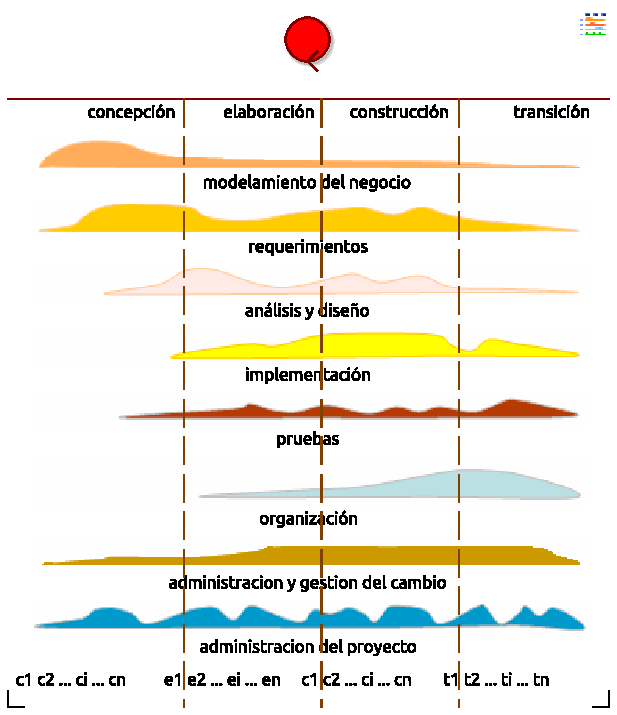
\includegraphics[width=0.7\linewidth]{proyecto/metodologia/imgs/rup}
	\caption{Proceso RUP \cite{SBol,Bas,Bab,Arc}}
\end{figure}


%\lstinputlisting[language=java]{C:/a/Cliente.java}


\part{DISEÑO}
\chapter{Requerimientos}
\section{Introducción}
cntenido...
\newpage
\chapter{Interacción}
\section{Introducción}
cntenido...
\newpage
\chapter{Diagrama de clases}
Los diagramas de clase son una de las herramientas UML más utilizadas para el diseño de software, ya que mediante ellos se puede demostrar la manera en que interactúan las distintas clases de un programa entre sí, además de la manera de ver la manera en que interactúan con el programa.
\begin{figure}[h!]
	\centering
	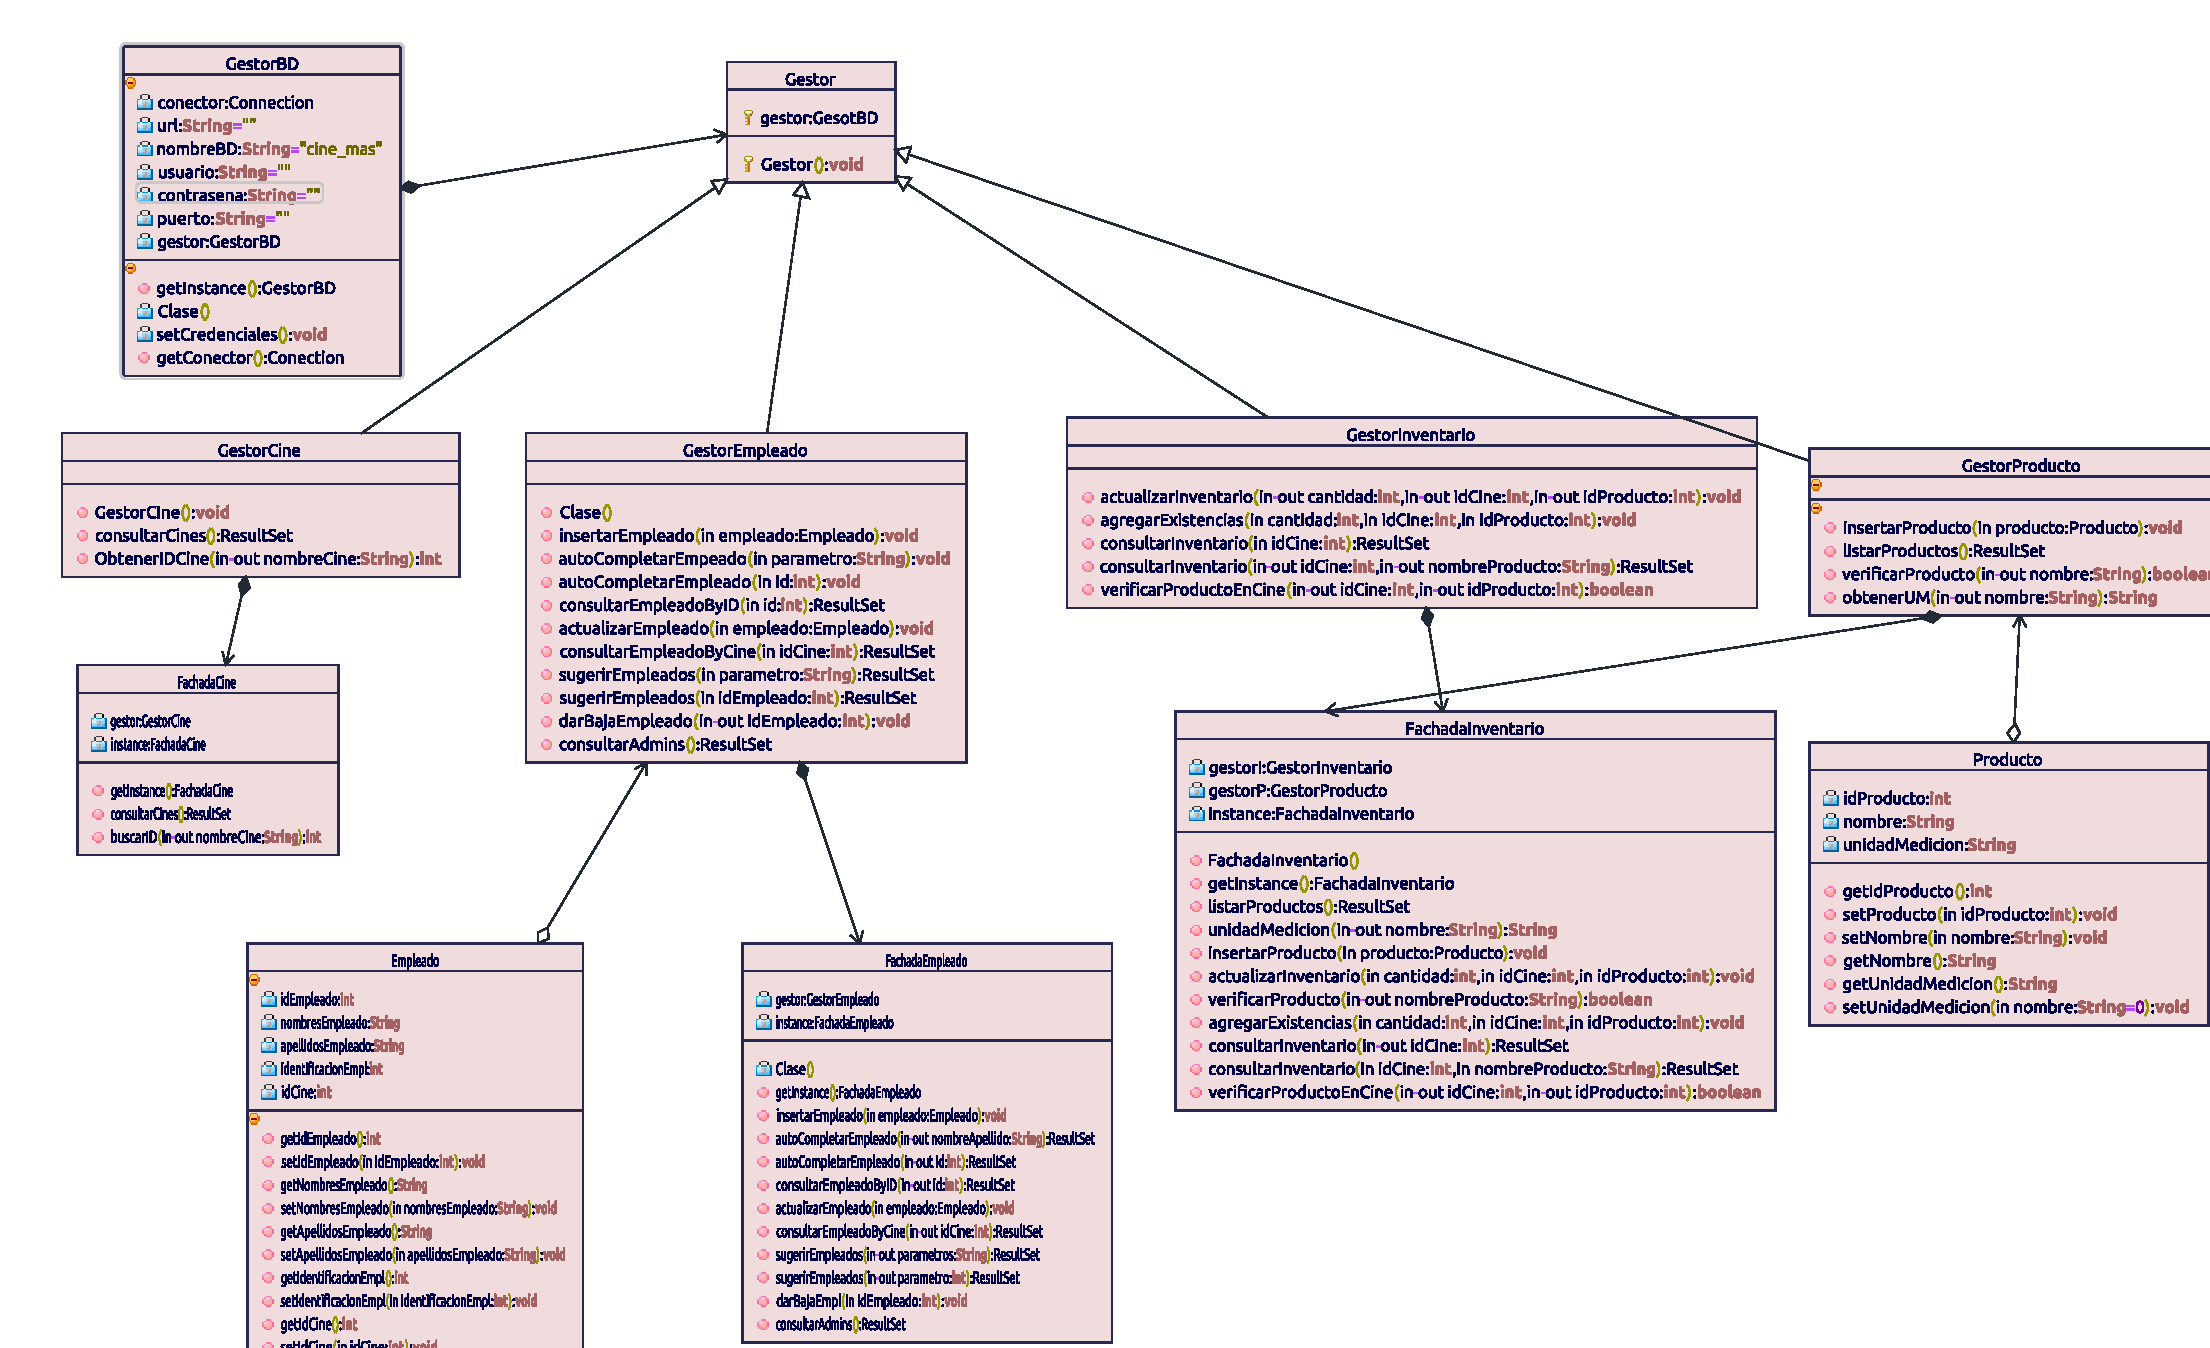
\includegraphics[scale=0.4]{diseno/clases/imgs/clases}
	\caption{Diagrama de clases}
\end{figure}
Las clases están conformadas por tres partes importantes: el nombre de clase, los atributos y las operaciones.

\subsection{NOMBRE DE CLASE:}
En esta sección es donde se define la clase, generalmente se nombran con sustantivos y se busca, mediante estos expresar de manera implícita lo que representa la clase.
  
\subsection{ATRIBUTOS}
Son las características propias de la clase, los elementos que la hacen única. Todos los atributos tienen ciertas características especiales que determinarán la manera con la que se interactúa con ellos.

\subsubsection{VISIBILIDAD}
Cuando hablamos de la visibilidad de un atributo se hace referencia a facilidad que tienen otras clases de ver los atributos de una clase en específico, existen cuatro tipos de visibilidad.

\begin{itemize}
	\item{\textbf{Privada:} este tipo hace referencia a que la única clase que tiene acceso a un atributo es la clase dueña del atributo.}
	\item{\textbf{Protegida:} este tipo está fuertemente ligado con la herencia, pues significa que los atributos son privados para todas las clases excepto aquellas que extiendan de la clase que tenga el atributo protegido.}
	\item{\textbf{Paquete:} este tipo indica que el atributo es privado para todas las clases que no pertenezcan al mismo paquete del atributo dueño del atributo. 	}
	\item{\textbf{Pública:} finalmente este tipo indica que cualquier clase existe puede ver el atributo de la clase.}
\end{itemize}

\subsubsection{ALCANCE}
Esta característica de los atributos nos indica el lugar que va a ocupar en memoria, partiendo del hecho de que en todo programa se cuenta con tres tipos de memoria: memoria estática, memoria de pila, memoria de montículo.

\begin{itemize}
	\item{\textbf{Memoria estática:} Esto nos indica que un atributo no puede cambiar en tiempo de ejecución, es decir, siempre tendrá el mismo valor.}
	\item{\textbf{Memoria de pila:} la mayoría de los atributos se encuentra en esta memoria, son datos que cambian constantemente.}
	\item{\textbf{Memoria de montículo} En esta memoria se encuentran todos los atributos que necesitan ser instanciados, generalmente con la palabra reservada \textbf{new}}
	
\end{itemize}

\subsubsection{PROPIEDADES}
Esta característica de los atributos es lo que nos indica la posibilidad que se tiene de ser modificados en tiempo de ejecución, se tienen de do tipos: Final y volátil.

\begin{itemize}
	\item{\textbf{Final o Constante:} ste tipo de atributo es un atributo que una vez definido no puede ser modificado en tiempo de ejecución.}
	\item{\textbf{Volátil:} Por otro lado esta propiedad indica que el atributo puede ser optimizado en tiempo de ejecución.}
\end{itemize}

La definición de un atributo dentro de una clase se realiza de la siguiente manera:

\centerline{\textbf{\underline{Visibilidad nombre [ ]: tipo = valor {propiedad}}}}
Donde los “[ ]” hacen referencia a la cantidad de elementos que se tienen y el subrayado al alcance que tienen dichos atributos.



\subsection{OPERACIONES}
Cuando se habla de las operaciones de una clase se hace referencia a las “habilidades” que esta tiene para poder interactuar con el programa, al igual que los atributos tiene ciertas características que las diferencian las unas de las otras.


\subsubsection{VISIBILIDAD}
La visibilidad de una operación es muy parecida con la visibilidad de los atributos, con la diferenciación de que en general solo cuenta con visibilidad pública y privada. 

Para saber si una operación es pública o privada hay que tener un término que se llama cohesión secuencial, es decir, si la operación necesita de otras operaciones para funcionar correctamente.

Una operación es privada si dicha operación  realiza una actividad que solamente tiene sentido dentro de la clase.

una operación es pública si la operación permite la interacción con otras clases. Generalmente dentro de ella aparece la cohesión secuencial, es decir, ella llama a las operaciones privadas de la clase. Se denomina interfaz, pues es un mediador con otras clases.


\subsubsection{PROPIEDADES}
En el caso de las operaciones las propiedades indican el tipo de acción que permite realizar.

\begin{itemize}
	\item{\textbf{Final: }La operación no permite sobrecarga, es decir, las clases hijas no podrán utilizarla.}
	\item{\textbf{Query: }Es una operación que no permite modificaciones, los atributos de la clase no son modificables.}
	\item{\textbf{Modify: }indica que la operación tiene la habilidad de modificar de manera permanente los atributos de la clase.}
	\item{\textbf{Synchronized: }Esta propiedad tiene sentido cuando se habla de hilos, pues determina que un hilo no pasará la responsabilidad hasta no haber terminado el proceso.}
\end{itemize}


\subsubsection{PARÁMETROS}
Los parámetro son la información que recibe la operación para poder realizar el proceso asignado, tienen una dirección que indica la característica del atributo:

\begin{itemize}
	\item{\textbf{in:} El atributo se pasa por valor.}
	\item{\textbf{out:} el parámetro será retornado.}
	\item{\textbf{in-out:} el parámetro se pasa por referencia. }
\end{itemize}

La manera en que se escriben las operaciones dentro de una clase es la siguiente:

\centerline{\textbf{\underline{Visibilidad nombre (parámetros): retorno {propiedad}}}}


\subsection{RELACIONES}
Estas relaciones tienen la característica de tener reuso de caja negra, es decir que las clases que se relacionan mediante ellas no tienen conocimiento de cómo se lleva a cabo una operación, pero aún así pueden hacer uso de ellas. Por otro lado, tienen el problema de que tienen un acoplamiento muy alto, lo que significa que la necesidad entre las clases es algo muy elevado.

\subsubsection{Cliente/proveedor}
Estas relaciones se dividen en dos grandes subramas: Dependencias y Asociaciones.

\textbf{Dependencia:}
Estos casos se dan cuando una clase utiliza otra clase para poder llevar a cabo una función (include, call, instance of, etc).

\textbf{Asociación:}
Esta tiene de dos tipos, el primero, la agregación, indica que la relación entre ellos no es vital, es decir, el cliente puede vivir sin el proveedor. Por otro lado la composición indica una relación vital, es decir, el cliente no puede vivir, ni tener sentido a no ser que tenga al proveedor.


\subsubsection{Generalización/Implementación}
Estas relaciones tienen la característica de tener reuso de caja blanca, es decir que las clases que se relacionan mediante ellas  tienen conocimiento de cómo se lleva a cabo una operación, e incluso pueden llegar a modificarlo. Por otro lado, tienen la ventaja de que tienen un acoplamiento muy bajo, lo que significa que la necesidad entre las clases es algo que puede pasar a segundo plano.

Por un lado las generalizaciones permiten crear una clase a partir de otra, con las mismas características, pero con la idea de que tenga un rol diferente. Por otro lado las implementaciones indican el uso de algunas operaciones de una interfaz en una clase determinada.

\begin{figure}[h!]
	\centering
	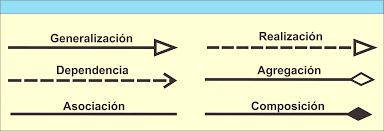
\includegraphics[scale=0.4]{diseno/clases/imgs/relaciones}
	\caption{Relaciones entre clases}
\end{figure}

\chapter{Patrones de diseño}
Para la estructuración del proyecto en curso se contemplaron los siguientes patrones de diseño:
\leavevmode
\linebreak
\begin{itemize}
	\item{\textbf{Abstract Factory:} Abstract Factory es un patrón de diseño que provee una interfaz para la creación de familias de objetos o objetos dependientes relacionados entre sí sin especificar sus clases concretas.
	\begin{figure}[h!]
	\centering
		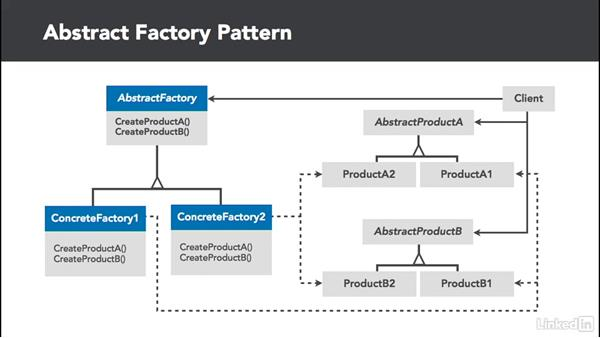
\includegraphics[scale=0.8]{diseno/patrones/imgs/abstractfactory}
		\caption{Patrón de diseño 'Abstract Factory'}
	\end{figure}
	Concretamente, se busca implementar este patrón de diseño para otorgar flexibilidad al momento de querer migrar todas operaciones y consultas de la base de datos a otro DBMS. Para este proyecto inicialmente se está trabajando con el DBMS PostgreSQL, pero si se quisiera migrar a otro tal como Oracle, MySQL u otro, este patrón otorga flexibilidad y facilidad para hacerlo. Para implementarlo, se parte de la base de que las operaciones sobre la base de datos se pueden ver como una familia de dos objetos: una conexión y un gestor. La conexión transportará todas las operaciones al DBMS que el gestor le solicite.
	\begin{figure}[h!]
	\centering
		\includegraphics[scale=0.7]{diseno/patrones/imgs/abstractfactoryDBMS}
		\caption{Patrón de diseño 'Abstract Factory' implementado dentro del proyecto}
	\end{figure}}
	\item{\textbf{Facade:} El patrón de diseño fachada provee una interfaz unificada para un conjunto de interfaces en un subsistema.
	\begin{figure}[h!]
	\centering
		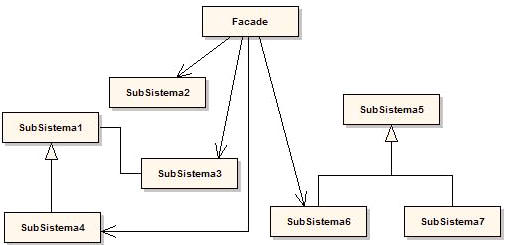
\includegraphics[scale=0.5]{diseno/patrones/imgs/facade}
		\caption{Patrón de diseño 'Facade'}
	\end{figure}	
	En el patrón de diseño 'Abstract Factory' que se planteó en el punto anterior, la interacción de la base de datos se da por medio de la clase 'DBFactory', que hace el papel de fábrica de los componentes que permiten dicha conexión; pero aquellos clientes que deseen interactuar y realizar operaciones con dicha conexión no deberían tener una relación con la clase 'DBFactory', de tal manera que se plantea el uso de una \textbf{Fachada} que establezca una interfaz que sirva de intermediaria entre ambas partes.
	\begin{figure}[h!]
	\centering
		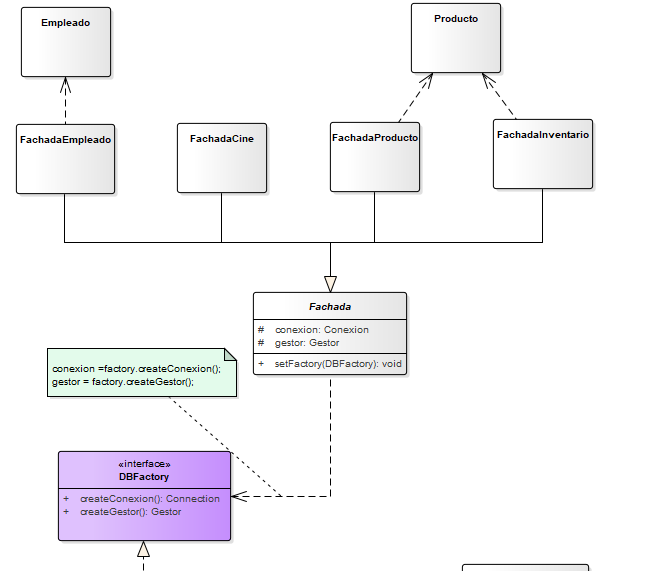
\includegraphics[scale=0.7]{diseno/patrones/imgs/facadeimplementado}
		\caption{Patrón de diseño 'Facade' implementado}
	\end{figure}
	}
	\item{\textbf{Singularidad (Patrón Prs):} El patrón de diseño de singularidad es un patrón -R el cuál es una mejora para la implementación relacionanda con el patrón singletón, con la ventaja de que mediante este patrón se pueden heredar todas las caraterísticas y ventajas que ofrece la clase padre.	
	\begin{figure}[h!]
	\centering
		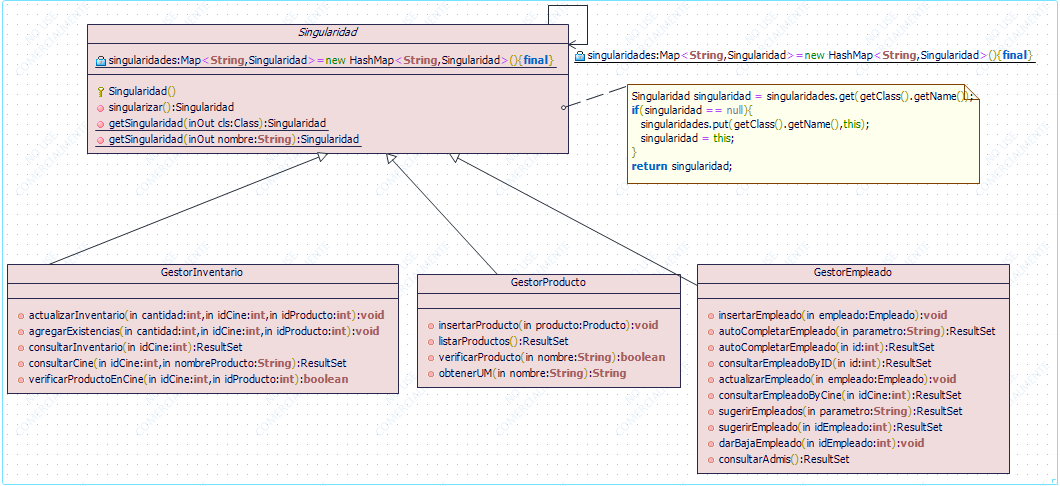
\includegraphics[scale=0.5]{diseno/patrones/imgs/singularidad}
		\caption{Patrón de diseño 'Singularidad' implementado}
	\end{figure}}
	
	 
\end{itemize}
\chapter{Estados}
\section{Introducción}
cntenido...
\newpage
\chapter{Componentes}
\section{Introducción}
cntenido...
\newpage
\chapter{Diagrama de Nodos}
\section{Definición}
Un Diagrama de Nodos modela la arquitectura en tiempo de ejecución de un sistema. Esto muestra la configuración de los elementos de hardware (nodos) y muestra cómo los elementos y artefactos del software se trazan en esos nodos.

\subsection*{Nodo}
Un Nodo es un elemento de hardware o software. Esto se muestra con la forma de una caja en tres dimensiones, como a continuación.

\subsection*{Instancia de Nodo}
Una instancia de nodo se puede mostrar en un diagrama. Una instancia se puede distinguir desde un nodo por el hecho de que su nombre esta subrayado y tiene dos puntos antes del tipo de nodo base. Una instancia puede o no tener un nombre antes de los dos puntos. El siguiente diagrama muestra una instancia nombrada de una computadora.

\subsection*{Asociación}
En el contexto del diagrama de despliegue, una asociación representa una ruta de comunicación entre los nodos. El siguiente diagrama muestra un diagrama de despliegue para una red, mostrando los protocolos de red como estereotipos y también mostrando multiplicidades en los extremos de la asociación.

\subsection*{Nodo como contenedor}
Un nodo puede contener otros elementos, como componentes o artefactos. El siguiente diagrama muestra un diagrama de despliegue para una parte del sistema embebido y muestra un artefacto ejecutable como contenido por el nodo madre (motherboard).

\section{Implementación}
Para el caso concreto del proyecto en desarrollo, se plantea una estructura de cliente-servidor a nivel de bases de datos; la información estará almacenada en una base de datos puesta en un servidor mientras que por  parte del cliente, existirán 2 herramientas cliente: una de tipo \textbf{Administrativa} y otra dirigida a los \textbf{Clientes finales}. Dichas herramientas se conectarán de forma remota al servidor para la interacción de los usuarios con la información. En la siguiente imagen se expone la implementación mencionada:

\begin{figure}[h!]
	\centering
	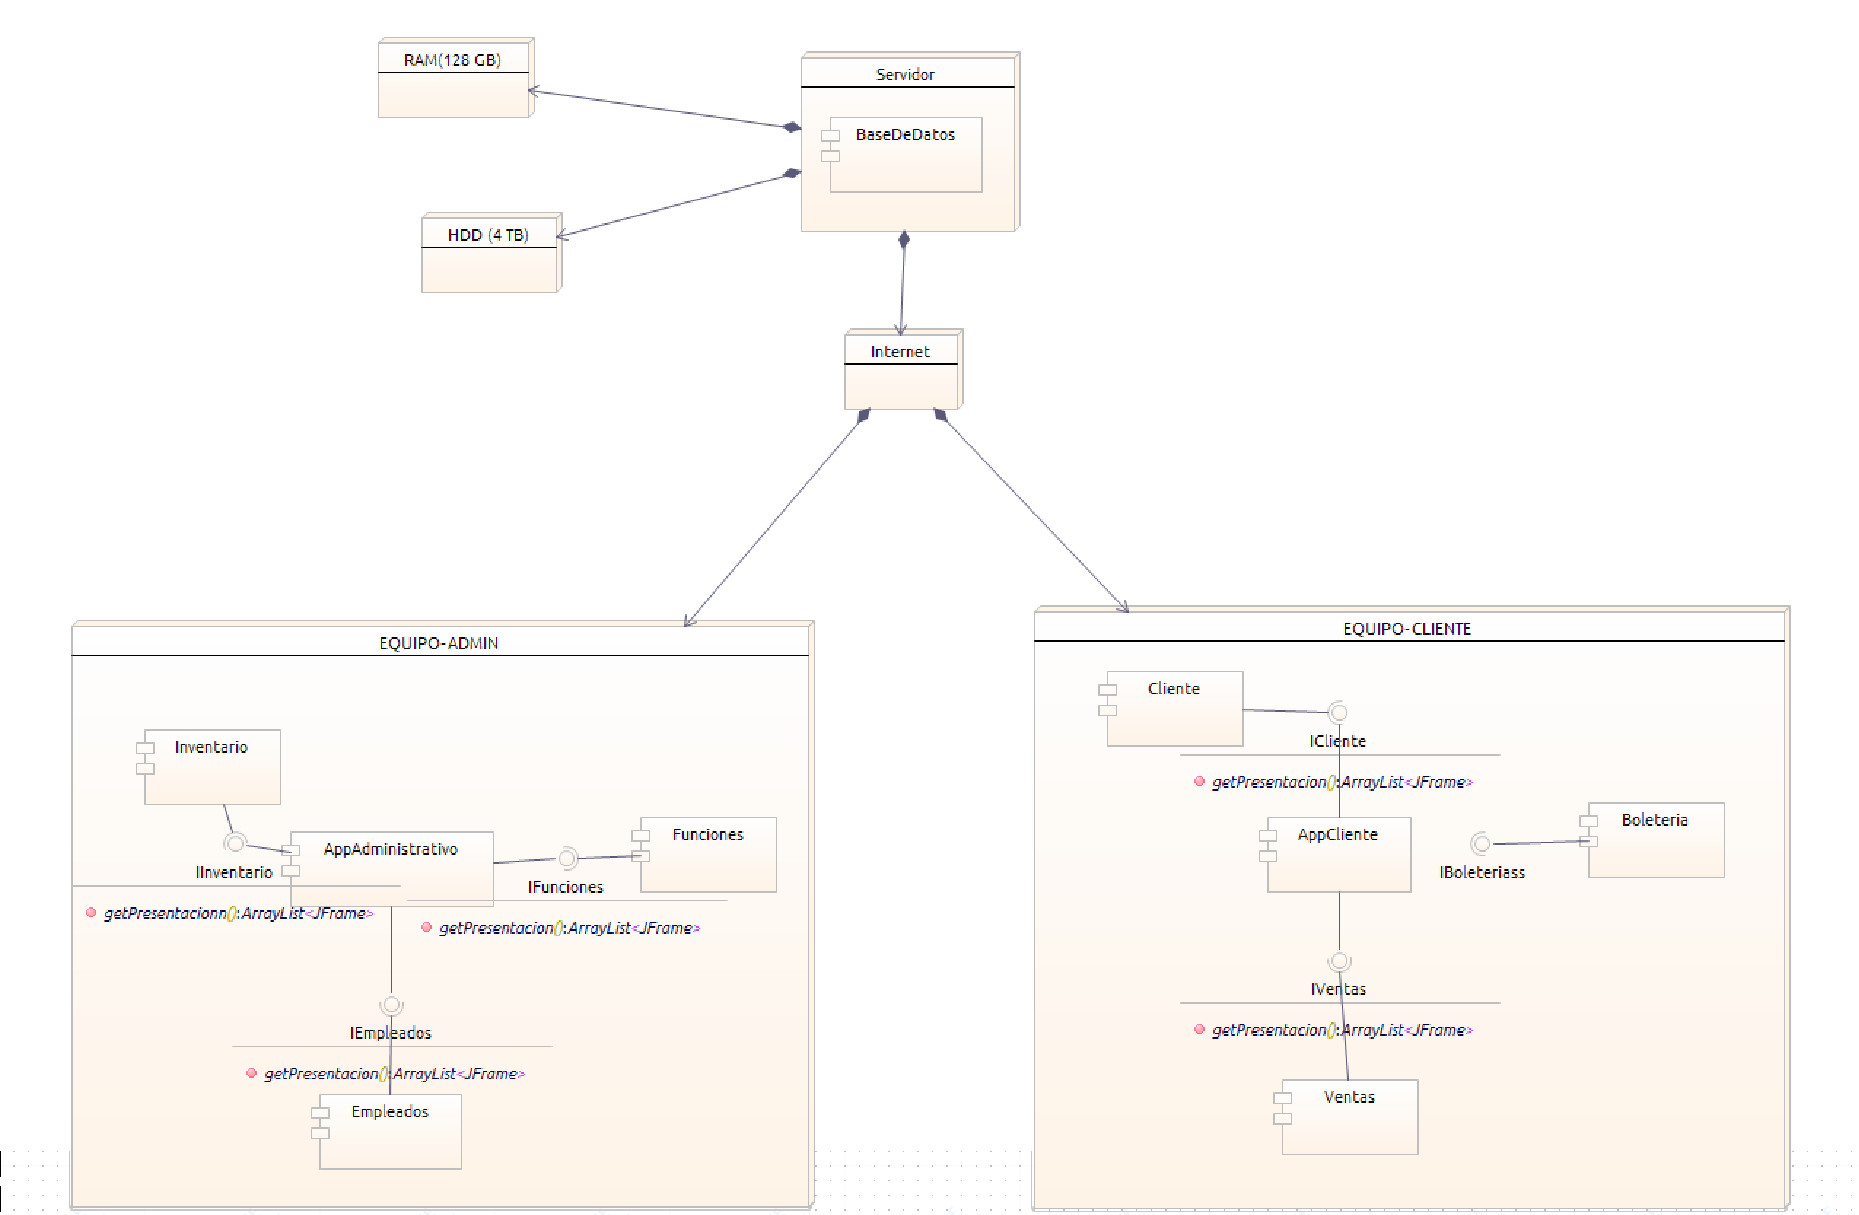
\includegraphics[scale=0.5]{diseno/nodos/img/diagramaNodos}
	\caption{Diagrama de Nodos}
\end{figure}

\chapter{Actividades}
\section{Introducción}
cntenido...
\newpage
\part{REFLEXIONES}
\chapter{Conclusiones}
\section{Introducción}
cntenido...
\newpage
%---bibliografia
\bibliographystyle{plain}
\bibliography{reflexiones/bibliografia/libros,reflexiones/bibliografia/articulos}

\end{document}